
\section{Computation, corpus, and robustness}\label{app:comp}

\subsection{Corpus and scoring}

The USPTO Trademark Annual Applications backfile (product TRTYRAP)
provides a complete record of US trademark filings from 1884 onward. The
deepest diagnostic work uses the complete software/electronics class
(Nice 009; 1.81M filings); the diffusion application uses four classes
totalling 2.32 million granted filings 1990--2024; the gate analyses use
all 45 classes. The firm-level panels link trademark owners to SEC EDGAR
financial filers and to PatentsView patent assignees by normalized-name
join.

The topic representation is a $T = 50$ LDA fit on a stratified sample of
448{,}437 filings across all 45 classes (vocabulary of 62{,}168 unigrams
and bigrams); every filing 1990--2024 is transformed to a dense 50-topic
distribution, and past-facing and future-facing surprise are computed against
per-filing topic references spanning 1{,}826 days on each side of the filing
date, scoring 1995--2019. A filing whose window holds fewer than 500
same-class filings on either side is left unscored, since a thin reference
inflates the divergence mechanically; that floor, together with the corpus
edges, is why roughly two-thirds of filings carry a score. A term-level variant is retained
alongside, on the same anchoring: token distributions (within-class
document frequency $\geq 50$) against per-filing windows of the same
1{,}826 days, Dirichlet-smoothed ($\alpha = 1$) over the class vocabulary.
Because a goods/services description runs to a few dozen words, the
divergence is needed only at the terms a filing actually uses, so the
reference is carried as a running count vector and read sparsely. The term
variant is used where vocabulary identity is the object (phrase transit)
and as the comparison scoring throughout. Both representations are also computed under an
exponentially decayed reference with a two-year half-life, truncated at the
same window; Appendix~\ref{app:scoring} reports what changes.

\subsection{Scores are interpretable from 1995}

\emph{Burn-in} is the span at each end of the corpus where the reference
windows cannot be filled, so scores there reflect a thin reference rather
than the text being scored.

The signal depends on having enough past and future filings to populate
the references; the 5-year past window is incomplete before 1990 and the
future window after 2020, and both zones are excluded
(Figure~\ref{fig:burnin}). The burn-in cut is set empirically: thin past
references inflate past-facing surprise, and profiling that bias across
all 44 sufficient-volume classes gives a median absolute bias of
$\sim$2.0 nats --- the natural-log unit in which these divergences are
measured --- in 1990, 0.25 in 1991, 0.10 in 1992, and 0.04 from 1993
onward, below any interpreted effect size. The 1995--1997 deviations
($\sim$0.15--0.17) are not burn-in --- mechanical contamination cannot
rebound --- but the dot-com era moving the corpus. Per-class burn-in
lengths estimated under a stability-band criterion track each class's
noise floor rather than its reference density, so a single standard cut
at 1995 is used, conservative by about two years.

\begin{figure}[h]\centering
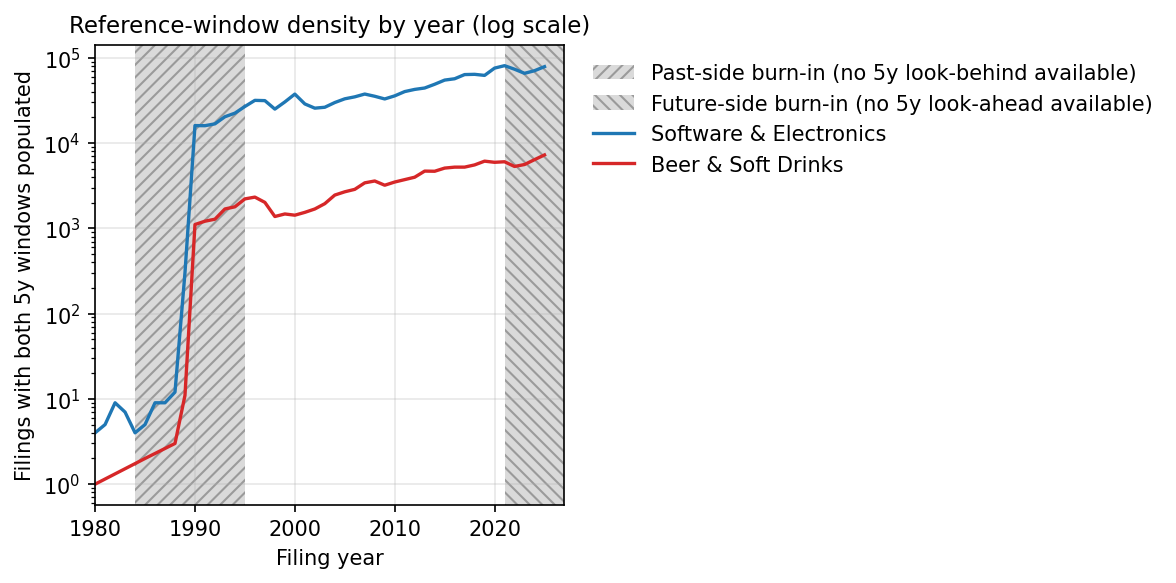
\includegraphics[width=0.85\textwidth]{results/burnin.png}
\caption{Reference-window density by year on log scale. Hatched regions
are the past-side and future-side burn-in zones where the 5-year window is
incomplete. The windows determine only how surprising a filing's language
is --- its score at the filing date. The outcome the score is tested
against is read separately and later: whether the registration survived
the use-proof gate, decided at registration age six to seven, which is why
the score is interpretable from 1995 but the gate sample ends with the
2018 cohort.}
\label{fig:burnin}
\end{figure}

\subsection{Lead is a small residual, and term scoring tracks length}

Past-facing and future-facing KL are highly correlated however scored. On the
complete class-009 corpus under the production scoring they correlate at
$r = +0.988$ ($n = 1{,}109{,}643$); under term scoring on class-year
references the figure is $+0.971$. The lead $L$ is therefore a small residual
of two large, stable quantities: both levels have a standard deviation near
$0.70$ nats about a mean of $1.46$, while $L$ has a standard deviation of
$0.109$ --- about a sixth of either level's spread. Only $1.2\%$ of the two
levels' combined variance survives into their difference. That is what makes $L$ sensitive to
anything that inflates the levels, and under term scoring the dominant
such thing is document length. Term-scored
atypicality correlates with log filing length at $-0.646$ in class 009 and
$-0.587$ in class 035, for the reason set out in Section~
ef{sec:construct}:
the divergence charges a filing for the narrowness of its own distribution, and
that narrowness is fixed by how many distinct terms it uses. Theme scoring
breaks the coupling, taking the same correlations to $-0.084$ and $+0.058$ ---
the second of them positive. The consequence for the lead is direct: the standard deviation
of $L$ rises threefold across deciles of $A$ under term scoring and by a
quarter to a half under topic scoring, so a unit of lead means roughly the
same thing everywhere only in the topic representation.
Appendix~\ref{app:representation} shows this as a length surface over the
two axes. Two qualifications. Topic scoring returns a finite value for about 65\% of
filings, so the two columns are not drawn from the same set; re-estimating the
term-scored correlations on exactly the topic-scored subset barely moves them,
which puts the contrast down to the representation rather than the sample. On
that common subset the spread comparison is nearer twofold than the threefold
quoted above. And ``flat'' means no
monotone length gradient rather than constant: class 035 under topic
scoring is mildly U-shaped in $A$. The two scorings agree only
moderately per filing (Pearson 0.46, Spearman 0.36 on 1.9M jointly
scored observations), which gives their agreement on the mark-level
patterns evidential force and their disagreement on the firm-level
patterns diagnostic force (Appendix~\ref{app:hazard}). Across
$W \in \{3, 5, 7\}$, 6.9--10.4\% of filings flip sign. Per-filing noise
attenuates at every aggregation used: firm-year means, token pools,
theme prevalence trajectories.

Alignment with expert innovation judgment is at most suggestive. Firms on
BCG/MIT ``most innovative'' lists sit $+0.09$ standard deviations above the panel mean
under term scoring ($p = 0.22$), $+0.14$ under topic scoring
($p = 0.07$), and $+0.08$ at $T = 200$ ($p = 0.20$). The matched
sample is 41 firms, which is too small to carry weight in either
direction, and the paper draws no inference from it. Patent counts remain
uncorrelated with \dkl{} on the same panel (Pearson $+0.010$).

\subsection{The mark-level results hold under every scoring}\label{app:scoring}

The snapshot cross-check on the single one-gate-elapsed cohort
(registrations 2016--2018, terminal status 710 versus 701--705/800)
agrees with the event-dated estimates and is scoring-robust: $-5.4$pp
survival across quintiles under topic scoring and $-5.7$pp under term
scoring on the identical sample (Figure~\ref{fig:s8pooled}). Under term scoring, gate survival
\emph{rises} in the raw KL level ($+6.5$pp past-facing, $+7.6$pp
future-facing): atypical text survives the use requirement better
while leading text survives it worse --- the same two-axis
separation as Section~\ref{sec:bluesea}, at the mark level.

\begin{figure}[h]\centering
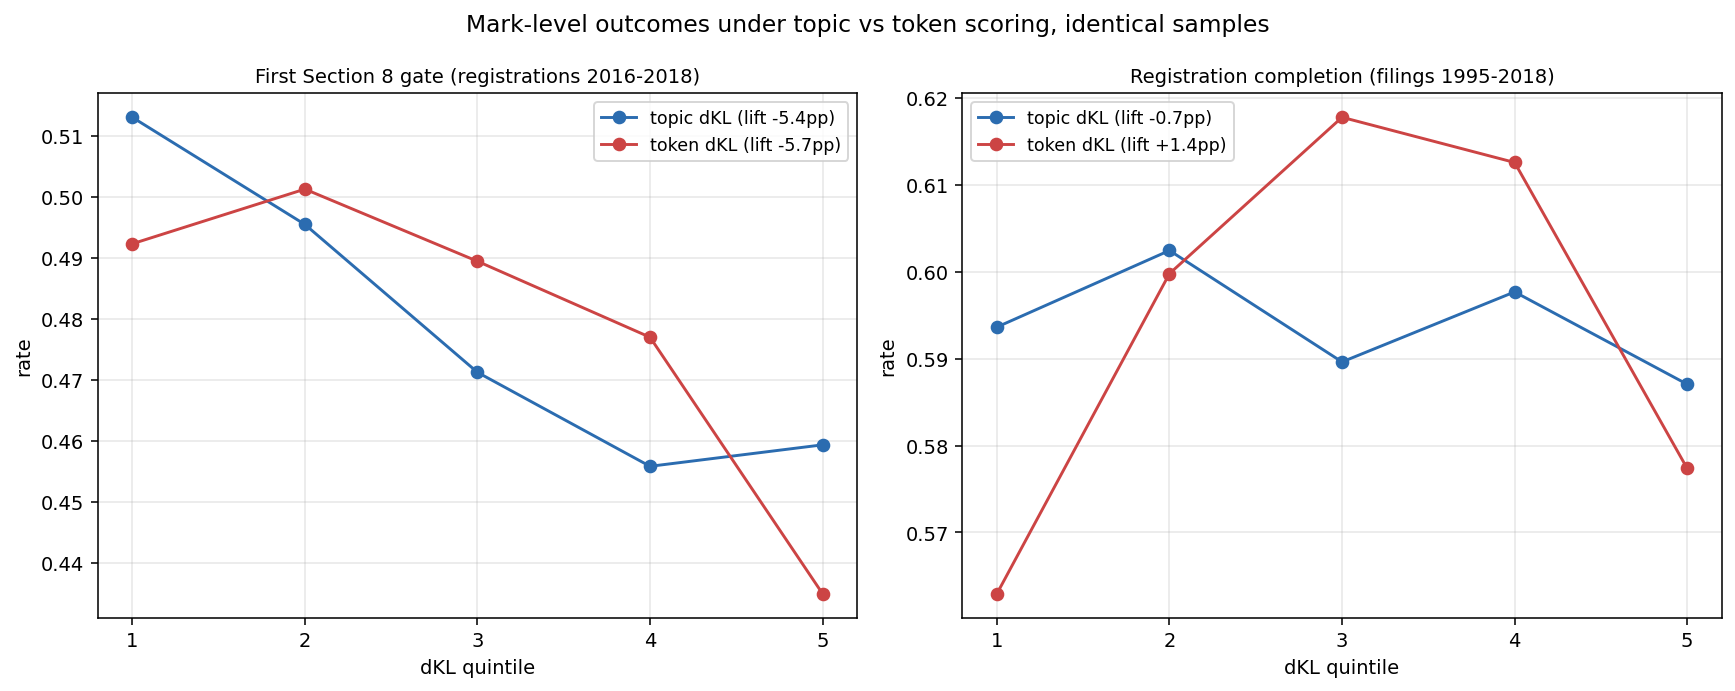
\includegraphics[width=\textwidth]{results/topic_outcomes_all.png}
\caption{The two mark-level outcomes under topic and term scoring on
identical samples, pooled across classes, by within-class lead quintile
(1 most lagging, 5 most leading). \emph{Left:} the share of registrations
2016--2018 that survived the first use-proof gate at years five to six,
read from terminal status codes, where the two representations agree
closely. \emph{Right:} registration completion
(filings 1995--2018), where they do not: the inverse-U in the signed axis
is present under term scoring (depth $+0.048$) and absent under topic
scoring (depth $-0.001$). The gate result is scoring-robust; the
registration curvature on this axis is not, and Section~\ref{sec:results}
reports only the unsigned version.}
\label{fig:s8pooled}
\end{figure}

\subsection{Annual reference buckets overstate the penalty by a third}\label{app:rolling}

Every estimate uses a reference anchored on the filing's own date. The
alternative is one reference per class-year, under which a filing made on 1
January and one made on 31 December receive identical references and neither
sees any of the language filed during its own year.
Appendix~\ref{app:choices} reports the calendar signature that leaves.

First, the gate penalty was overstated by about a third. On the same 3.10
million registrations, the top-versus-bottom contrast is $+2.15$pp
(SE $0.30$) under annual buckets and $+1.39$pp (SE $0.17$) under per-filing
windows. The attenuation is remarkably uniform across specifications ---
the ratio runs $0.59$ to $0.73$ for every sample split in
Table~\ref{tab:gate_lpm} --- and it is an attenuation of magnitude only:
standard errors fall by roughly half, so the $t$-statistic \emph{rises},
from $7.2$ to $8.3$. The same holds in the software class alone, where the
contrast moves from $+7.40$pp to $+5.25$pp.

Second, the shape of the gate penalty changes. Under annual buckets the
quintile profile looked like a gradient with a steeper final step; under
per-filing windows the gradient through the interior quintiles is shallower
and the final step dominates, with the top quintile carrying about seventy
percent of the total.
The coarser measure spread a top-quintile effect across the whole range.

Third, one published shape does not survive. Registration completion showed
an inverse-U on both the unsigned and the signed axis. Only the unsigned one
is real; on \dkl{} the curvature disappears entirely under per-filing
windows, and the earlier interior peak is attributable to the month
gradient above. The firm-level results are the least affected by the window change,
though they are sensitive to the owner-to-registrant linkage instead
(Section~\ref{sec:bluesea}): the signed decomposition keeps both its signs
and its significance under either window.

\subsection{Signal is flat between five and seven years}\label{app:wsweep}

The window is a parameter of the measure, not a property of it, and the five
years used throughout was inherited from the class-year construction rather
than chosen under the current one. Re-scoring the software class at several
widths under per-filing references, and judging each by the first-gate
quintile contrast it produces, gives $+2.02$pp at two years, $+2.20$ at
three, $+3.23$ at five and $+3.37$ at seven, each on an identical sample of
452{,}911 registrations and each with a standard error of $0.23$pp. Signal
rises steeply from two to five years and is flat between five and seven: the
$+1.03$pp gain from three to five is well outside the sampling error, the
$+0.14$pp from five to seven is not. A ten-year window returns $+2.89$pp,
but that figure is not comparable to the others --- requiring both windows
to lie inside the corpus costs 22\% of the scored filings and 13\% of the
gate sample, dropping the earliest and latest registration years, which are
also the years whose contrasts differ most. The apparent decline at ten
cannot be separated from that change in composition and is not evidence
about window width. On the range where the sample is fixed, seven years is
nominally the peak and five is within noise of it while retaining more of
the corpus, so five is defensible rather than optimal. The sweep is on one class
and one outcome.

\subsection{The gate punishes breaking with the past more than resembling the future}\label{app:wmix}

``Leading'' is relative to a reference, and the two references need not be
the same width. A short past and a long future make lead a measure of
foresight --- whether the filing resembles where the class was heading over
the next seven years more than what it wrote in the last three. A long past
and a short future make it a measure of rupture --- whether the filing has
broken with what the class had established over seven years, judged against
only the next three. Scoring every class on the production representation
and per-filing windows at $W \in \{3, 5, 7\}$ years on each side, and
evaluating all five variants on the identical 3.10 million registrations
with quintiles assigned within class$\times$registration-year:

\begin{center}\small
\begin{tabular}{llrrrr}
\toprule
Variant & Past, future & \multicolumn{2}{c}{First-gate failure} & \multicolumn{2}{c}{Registration} \\
 & (years) & Q5$-$Q1 (pp) & classes $>0$ & Q5$-$Q1 (pp) & Q3 $-$ tails \\
\midrule
Foresight     & 3, 7 & $+1.65$ (0.09) & 31 of 44 & $+1.09$ & $+0.50$ \\
Symmetric     & 3, 3 & $+1.69$ (0.09) & ---      & $+0.79$ & $+0.13$ \\
Symmetric     & 5, 5 & $+2.29$ (0.09) & 33 of 44 & $+0.71$ & $+0.28$ \\
Symmetric     & 7, 7 & $+2.58$ (0.09) & ---      & $+0.48$ & $+0.65$ \\
Past-rupture  & 7, 3 & $+3.00$ (0.09) & 37 of 44 & $+0.01$ & $+0.33$ \\
\bottomrule
\end{tabular}
\end{center}

\noindent The symmetric five-year row is the paper's FE-only estimate in
Table~\ref{tab:gate_lpm}, reproduced here to the decimal, which fixes the
scale. The penalty rises monotonically along the mix, from $+1.65$pp under
foresight to $+3.00$pp under rupture, and rupture is the more pervasive
variant, positive in 37 of 44 classes against 31. In software the two are
$+1.82$ and $+5.07$pp. So the use requirement punishes distance from the
class's established language more than it punishes resemblance to its
coming language; but foresight carries a penalty of its own, more than half
the symmetric one, and the separation is a matter of degree rather than
kind.

Registration is a different matter. On the signed axis the top-to-bottom
contrast is at most a point on a 57\% base and the interior-minus-tails
depth at most two thirds of a point, under every mix. An earlier version of
this decomposition, run on the retired term-level calendar-year scoring,
found a registration inverse-U of four to five points that the window mix
did not touch; under per-filing references that curvature is gone on the
signed axis, consistent with Appendix~\ref{app:rolling}, which traces it to
the calendar artefact. The examiner's response to lead, on this scoring, is
close to nil.

\section{Representation and resolution drive the score; weighting does not}\label{app:choices}

\subsection{Representation, anchoring, weighting: which of the three matters}

A scoring is fixed by two choices. The \emph{representation} is what the
language is turned into: a distribution over 50 fitted topics, or a
distribution over the class vocabulary's terms. The \emph{reference} is what
that is compared against, and it hides two sub-choices --- the
\emph{anchoring} (one reference per class-year, or one per filing built on its
own date) and the \emph{weighting} inside the window (every day equal, or
decaying by half every two years). Six builds exist:

\begin{center}\small
\begin{tabular}{lllrr}
\toprule
Representation & Anchoring & Weighting & sd(lead) & sd(atypicality) \\
\midrule
Topics & class-year & flat          & $0.132$ & $0.672$ \\
Topics & per-filing & flat          & $0.102$ & $0.698$ \\
Topics & per-filing & half-life 2y  & $0.082$ & $0.698$ \\
Terms  & class-year & half-life 2y  & $0.299$ & $1.330$ \\
Terms  & per-filing & flat          & $0.155$ & $1.101$ \\
Terms  & per-filing & half-life 2y  & $0.130$ & $1.102$ \\
\bottomrule
\end{tabular}
\end{center}

\noindent All six are compared on the 6.01 million filings every one of them
scored. The second row is the production scoring. The fourth is the legacy
build, and it is the one to handle carefully: it moves anchoring \emph{and}
weighting at once, so a result computed on it cannot be attributed to either.
That is why the two per-filing term builds were constructed.

Changing one choice at a time settles the ordering. Correlations of lead
between builds differing in exactly one respect:

\begin{center}\small
\begin{tabular}{lrr}
\toprule
Choice varied & $r$ (lead) & $r$ (atypicality) \\
\midrule
Weighting, flat vs half-life 2y (topics)  & $0.982$ & $1.000$ \\
Weighting, flat vs half-life 2y (terms)   & $0.970$ & $1.000$ \\
Anchoring, class-year vs per-filing (topics) & $0.738$ & $0.929$ \\
Resolution, 50 vs 200 themes              & $0.636$ & $0.828$ \\
Representation, topics vs terms           & $0.460$ & $0.396$ \\
\bottomrule
\end{tabular}
\end{center}

\noindent The weighting is close to irrelevant: whether recent language counts
for more than distant language within the window barely moves the score, and it
does not move atypicality at all to three decimals, which is what the
$45$-degree rotation of Section~\ref{sec:construct} implies --- the long axis is
a property of the filing and the weighting acts almost entirely on the small
residual. Anchoring matters moderately. Resolution and representation matter
most: quadrupling the number of themes leaves the two builds agreeing on 40\%
of the variance in lead, and topics against terms on less than a quarter. A
robustness check that varies only the weighting is therefore close to a
restatement; one that varies the representation or the resolution is a real
test, which is why the term-scored replication in Appendix~\ref{app:scoring}
and the sweep below are the ones the claims lean on.

\subsection{Fifty themes is coarse, and the finding does not depend on it}

Fifty themes over a 62,168-term vocabulary is roughly one theme per industry,
so the partition is coarse enough that a reader may reasonably suspect the
findings belong to it. Raising the theme count does not add coverage --- the
vocabulary is fixed, and a larger $T$ re-partitions the same words --- but it
changes what counts as sitting far from an industry, and could change any sign.
Re-fitting the model at four resolutions on the same stratified sample and the
same analyzer, and re-scoring the software class under per-filing windows:

\begin{center}\small
\begin{tabular}{rrrrr}
\toprule
Themes & Gate contrast, lead & $t$ & Gate contrast, atypicality & $r$ with $T=50$ \\
\midrule
$50$   & $+3.23$pp & $13.8$ & $-14.01$pp & --- \\
$100$  & $+2.71$pp & $11.6$ & $-13.69$pp & $0.690$ \\
$200$  & $+5.20$pp & $22.2$ & $-13.45$pp & $0.640$ \\
$500$  & $+5.69$pp & $24.3$ & $-14.49$pp & $0.641$ \\
\bottomrule
\end{tabular}
\end{center}

\noindent Three readings, in descending order of how much weight they carry.
The sign and the significance are untouched across a tenfold change in
resolution, and so is atypicality, which stays within a point of $-14$pp
throughout. The magnitude is not: the lead contrast runs from $+2.71$ to
$+5.69$pp and does not move monotonically in $T$, so no single resolution can
be quoted as the software class's effect, and the figure this paper reports at
$T = 50$ sits at the low end of that range rather than the high one. And
agreement with $T = 50$ settles at $0.64$ without decaying as $T$ grows, which
says the resolutions share a fixed core and differ in the remainder rather than
drifting apart as the partition refines.

The corpus-wide contrast is steadier than the single class: at $T = 200$,
scored for all 45 classes, it is $+2.23$pp against $+2.29$pp at $T = 50$. Only
those two resolutions exist corpus-wide, so that is a two-point comparison, but
it is the one the paper's estimates run on, and pooling evidently averages away
much of the per-class resolution sensitivity.

\subsection{Two fits at one resolution disagree almost as much as two resolutions}

The sweep leaves one question open. Scores at different resolutions agree at
$r = 0.64$ to $0.69$ on lead, and neighbouring resolutions agree no better than
distant ones. That has two readings. The number of themes may genuinely change
what is being measured. Or a topic-model fit may simply be unstable --- two
runs settle in different local optima --- in which case the sweep is measuring
fitting noise and the resolution has little to do with it.

Holding $T$ fixed and moving only the seed separates the two. A second fit at
$T = 200$ on the same sample, the same vocabulary and the same number of
passes, differing from the first in nothing but its random seed, agrees with
it at $r = 0.79$ on lead and $r = 0.87$ on atypicality across 1.11 million
scored software-class filings. The cross-resolution figures were $0.64$ and
$0.83$. Most of what the sweep showed as resolution sensitivity is therefore
present between two fits that differ only in the seed: for atypicality nearly
all of it, for lead well over half. The resolutions are not measuring
different things; each fit is a noisy draw on the same thing.

The estimate moves less than the scores do. On the identical gate sample, the
first-gate lead contrast is $+5.20$pp under the first seed and $+4.88$pp under
the second (SE $0.23$ each), and the atypicality contrast $-13.45$ and
$-14.38$pp. Two consequences follow. A single fit's lead score carries
measurement error of roughly a fifth of its variance, which attenuates every
coefficient on lead toward zero; the estimates in this paper are on the
conservative side of what a noiseless score would return. And the spread of
magnitudes across the resolution table above, which does not move
monotonically in $T$, should be read as a band about a third of a point wide
from fitting noise alone rather than as a property of any particular $T$.

Annual anchoring leaves a signature that per-filing anchoring does not. Mean
lead by calendar month of filing, in units of the build's own standard
deviation, has no reason to trend --- nothing about filing in December rather
than January makes a description more forward-looking:

\begin{center}\small
\begin{tabular}{llr}
\toprule
Representation & Anchoring & December $-$ January (sd) \\
\midrule
Terms  & class-year & $+0.169$ \\
Topics & class-year & $+0.041$ \\
Topics & per-filing & $-0.008$ \\
Terms  & per-filing & $+0.017$ \\
\bottomrule
\end{tabular}
\end{center}

\noindent A December filing sits eleven months further from its past reference
and eleven months nearer its future one, and under annual buckets that shows up
as position in the calendar. Under per-filing references it is gone.

The substantive claim does not depend on any of this. The first-gate contrast,
computed on the common sample, runs $+2.73$, $+2.71$, $+2.39$, $+4.05$, $+3.97$
and $+3.19$pp on lead across the six builds in the order tabulated above, and
$-7.75$ to $-6.17$pp on atypicality. Every sign holds; term scoring returns the
larger lead contrast, so the headline estimate is the conservative
representation.

\subsection{One gate is linear; the public-reporting profile is a U}

\begin{figure}[h]\centering
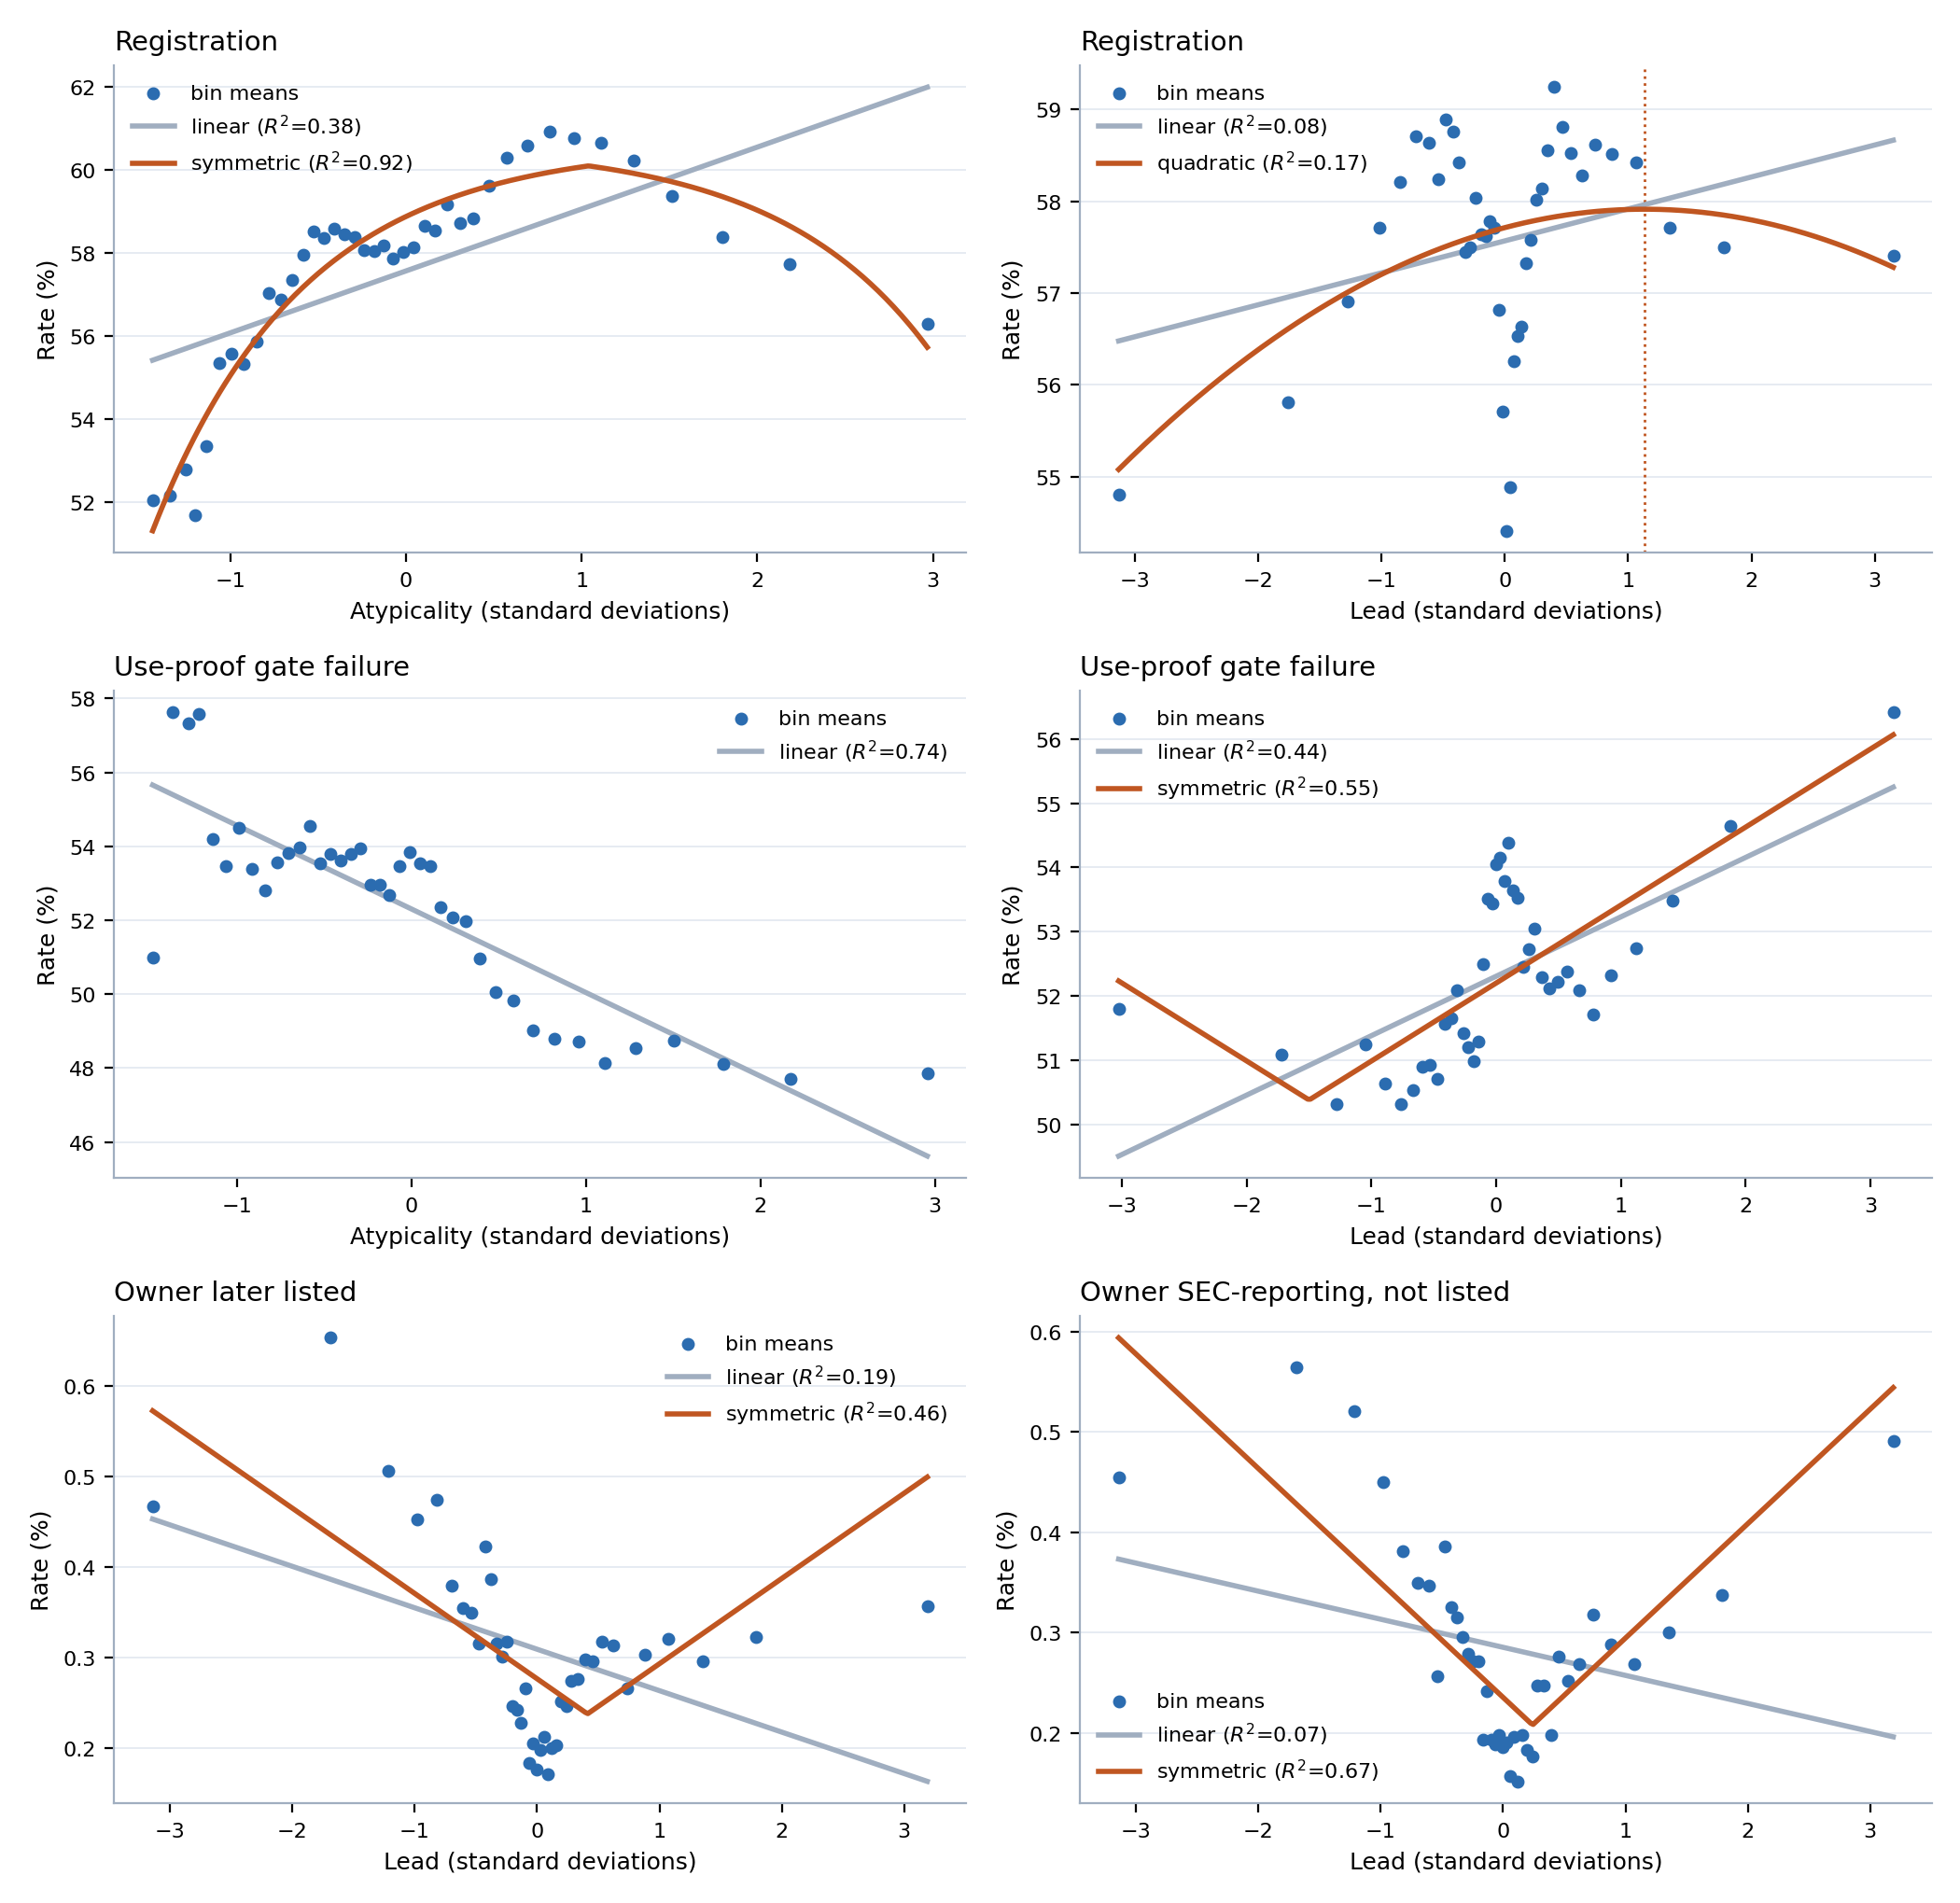
\includegraphics[width=\textwidth]{results/curve_shapes.png}
\caption{Binned profiles at the three gates, with the linear reading the
paper's contrasts assume and the shape selected by AIC where that is not
linear. Forty equal-count bins; the dotted line marks the fitted vertex. The
bottom row is the case that matters: a linear fit through the
public-reporting profile slopes downward while the data turn up at both tails.}
\label{fig:shapes}
\end{figure}

Four shapes were fitted to each profile by weighted least squares on 40
equal-count bins (Figure~\ref{fig:shapes}): linear, quadratic, an exponential
$a + b e^{cx}$, and a free-vertex symmetric form $a + b e^{c|x - x_0|}$ meant
to catch a U directly. Selection is by AIC.

\begin{center}\small
\begin{tabular}{llrrrl}
\toprule
Outcome & Axis & $R^2$ line & $R^2$ curve & $\Delta$AIC & Shape selected \\
\midrule
Registration & atypicality & 0.38 & 0.92 & 77.1 & curve, peak at $+1.04$ \\
Registration & lead & 0.08 & 0.17 & 1.9 & (quadratic; weak) \\
Use-proof & atypicality & 0.74 & 0.74 & 0.0 & linear \\
Use-proof & lead & 0.44 & 0.55 & 4.3 & V, vertex $-1.50$ \\
SEC reporting & atypicality & 0.74 & 0.84 & 15.2 & curve, peak at $+2.17$ \\
SEC reporting & lead & 0.13 & 0.59 & 26.3 & V, vertex $+0.30$ \\
\quad listed only & lead & 0.19 & 0.46 & 12.2 & V, vertex $+0.41$ \\
\quad reporting, not listed & lead & 0.07 & 0.67 & 37.2 & V, vertex $+0.24$ \\
\bottomrule
\end{tabular}
\end{center}

\noindent The winning form is a free-vertex $a + b\,e^{c|x-x_0|}$. On the
atypicality rows it is a genuine curve, with fitted exponents near $0.5$ to
$0.9$ --- a hump that peaks about one standard deviation above mean
atypicality at registration and about two above it at SEC reporting. On every
lead row the exponent collapses to the order of $10^{-4}$, which turns
$e^{c|x-x_0|}$ into $1 + c|x-x_0|$: what wins there is a \emph{V}, linear in
distance from a vertex. A V beating a parabola says the turn is sharper than a
quadratic allows, not that anything is multiplying. The script now flags that
degeneracy rather than leaving it to be read off the fitted constants.

Vertices are in standard deviations of the axis across filings. An earlier
version of this table standardized on the spread of the forty bin centres
instead, which is narrower than the filings' own spread and put the vertices
on a scale that did not match the per-standard-deviation slopes quoted
elsewhere in the paper.

The two rows for SEC reporting are the outcome Section~\ref{sec:bluesea} and
Table~\ref{tab:edgar} actually run on; the listed and reporting-only splits
below them show the same shape on each half, which is why the split does not
change the reading.

AIC here is computed on 40 binned means, not on the millions of underlying
filings, so it ranks shapes rather than testing them. The $77$ at registration
and the $12$ to $36$ at the public-reporting gates are decisive; the $1.9$ at
registration on lead and the $4.3$ at the use-proof gate are weak, and those
two rows are better read as ``no worse than linear'' than as curvature.

\subsection{Listing and merely reporting behave the same way}

``Appears in SEC records'' mixes two populations: companies whose shares trade, and entities that file with
the Commission without ever listing --- private issuers, funds, subsidiaries
registering securities. Splitting the 19{,}889 matched owner strings on whether
their CIK carries a ticker in the Commission's own company-ticker file gives
10{,}556 listed against 9{,}333 that file financial statements without one.

It does not change the finding. Among registered debut owners whose debut
filing is scored, $0.310$\% later appear as listed companies and $0.285$\% as
reporting non-listed ones, and both profiles are U-shaped in lead with vertices
at $+1.35$ and $+0.56$ standard deviations. The listed profile is slightly
flatter and noisier, which is what the smaller and more selected outcome
predicts. Whatever the signed axis is picking up at this margin, it is not an
artifact of counting non-operating registrants as commercial successes, and it
is not specific to the act of listing either.\footnote{Two limits on the split.
The ticker file is a current snapshot, so a company that listed in 2003 and was
acquired in 2011 appears in the non-listed tier; the tiers are therefore
``currently listed'' rather than ``ever listed,'' which will misclassify older
successes downward. And the base rates here are computed on the appendix's own
panel, which conditions on the debut filing carrying a score and so is smaller
than the body's sample.}

\section{The measurement hazard: term scoring manufactures firm-level signal}\label{app:hazard}

Under term-level scoring, leading filings appear to belong to
better firms. Among registered debut filings, the probability that the
owner ever appears in SEC EDGAR rises in term-\dkl{} from 0.29\% at the
bottom quintile to 0.42\% at the top; on an SEC-matched firm-year panel,
trailing 3-year mean term-\dkl{} predicts gross margin at $+2.3$pp per
standard deviation ($t = 2.7$ on the locally rebuilt panel through 2019; $+3.2$pp,
$t = 5.3$, on the published panel through 2024), with past-facing
surprise entering positively and future-facing negatively; and firm-year
term-\dkl{} predicts excess stock returns of $+1.5$ to $+5.0$pp per
standard deviation at one-to-four-year horizons. A larger debut-only return figure
($+28$pp at 4 years) fails a sample-size diagnostic and is not claimed.

None of the signed versions survives distribution scoring. On identical
samples, the debut listing gradient in signed topic-\dkl{} is flat to
declining, and the margin coefficient reverses: $-1.3$pp per standard deviation
($t = -1.8$) at $T = 50$, $-2.2$pp ($t = -3.1$) at $T = 200$, and
$-0.8$pp ($t = -1.1$) at $T = 500$, against the term-level $+2.3$pp;
the past-/future-facing decomposition flips sign and stays
flipped. The term-level listing gradient separately dissolves under
document-length controls: within length bands it is U-shaped rather than
rising, with the monotone rise contributed by composition across lengths
(listed firms' counsel write longer descriptions). The mark-level
results are unaffected --- they hold under both scorings at every
resolution.

Vocabulary blindness does not rescue the signed signal. The topic
model's vocabulary is sample-built, so rare and emergent terms are
invisible to it; if the firm signal lived exactly there, topic scoring
would erase a real signal rather than an artifact. Computing each
filing's invisible-vocabulary share (63.8\% of class-009 term
\emph{types} but only $\sim$9\% of token \emph{mass}): the share itself
is a strong firm marker (P(EDGAR) 2.9\% to 5.5\% across its quintiles;
gate survival $+5.7$pp), but \emph{within} invisible-share strata the
signed \dkl{} gradient on the firm outcome is flat to negative, while
the gate penalty holds in both strata ($-6.9$ and $-8.3$pp). The
term-level firm signal is \emph{unsigned specificity}: serious firms
describe specific products with specific, therefore rare, words, and
rare-term mass inflates term-\dkl{} mechanically. Topic count is a
partition dial, not a coverage dial --- a crypto/blockchain topic exists
at $T = 200$ but not at $T = 50$ or $T = 500$, because raising $T$
re-partitions the fixed vocabulary along dominant axes --- so resolution
sweeps test granularity, not coverage, and the invisible-share split is
the test that binds.

The registration filter does not explain the divergence. Dropping the
registration conditioning leaves the term-level listing gradient
essentially unchanged (0.26\% to 0.38\% across quintiles against 0.29\%
to 0.42\% conditional), and an examiner channel touching 4.3\% of failed
applications cannot generate several-point quintile gaps.

Term-resolved text-novelty measures can therefore manufacture
firm-performance correlations from drafting style and lexical specificity,
and a distribution-based rescoring is a cheap, decisive diagnostic.

\section{Examination rewards a middling specificity}\label{app:registration}

Across 3.59 million debut filings (57.6\% base rate), completion is an
inverse-U in \emph{atypicality}: it climbs from 46.6\% at the least atypical
end to about 58\% in the middle and falls back to 53.4\% at the most atypical
(Figure~\ref{fig:profiles}, panel C). The same shape appears on the
past-facing level alone, more mildly, running 54.0\% at the bottom quintile to
58.4--59.1\% in the middle and 57.7\% at the top (Figure~\ref{fig:outcomes}A).

The signed axis behaves differently. Completion on \dkl{} falls to a trough of
51.9\% just above the median and then rises steadily to 58.0\% at the leading
end. That trough is composition rather than timing: $|L|$ correlates with
atypicality at $+0.31$, so filings near zero lead are disproportionately
low-atypicality filings, which complete poorly for the reason above. Split by
atypicality, the trough is absent in the upper three fifths and survives in
the lowest. Reference windows built by calendar year put an inverse-U on this
axis too, but that one is an artifact of annual bucketing
(Appendix~\ref{app:rolling}) and does not survive at daily resolution. The
signed axis still enters a linear specification strongly
(Table~\ref{tab:staged}), but monotonically rather than through an interior
peak: what curvature exists at registration belongs to how far a filing's
language sits from its category, not to which side of it the filing sat.

The obvious objection is that unfamiliar language is simply refused more
often, so the measure recovers nothing beyond familiarity. Completion falls at
\emph{both} ends, so the most category-typical filings also complete less than
the middle, which familiarity cannot explain; and the curvature is specific to
the unsigned axis, the signed axis showing no interior peak at all.

Refiling after abandonment is itself mildly related to vocabulary position,
though not on the axis that matters here. Refiling rates are flat in
atypicality (a middle-minus-tails difference of $-0.06$pp on a 3.6\% base) but
rise with lead, from 2.6\% among the most lagging abandoned applications to
3.4\% among the most leading. Firms whose language ran ahead of their industry
are slightly likelier to try the same mark again.

\section{How refiled descriptions are rewritten}\label{app:refile}

Figure~\ref{fig:refile} shows the goods/services description before and
after a rewrite, for the 31{,}084 refilings in Section~\ref{sec:results}
whose text changed. A pair is an abandoned application and the same owner's
later registration of the identical mark in the same Nice class within six
years; the earliest registered refiling is kept. Counsel of record is read
from the prosecution history of each filing separately, so a pair can change
representation between attempts. Atypicality is on the production scoring;
length is the word count of the normalized description.

\begin{figure}[h]\centering
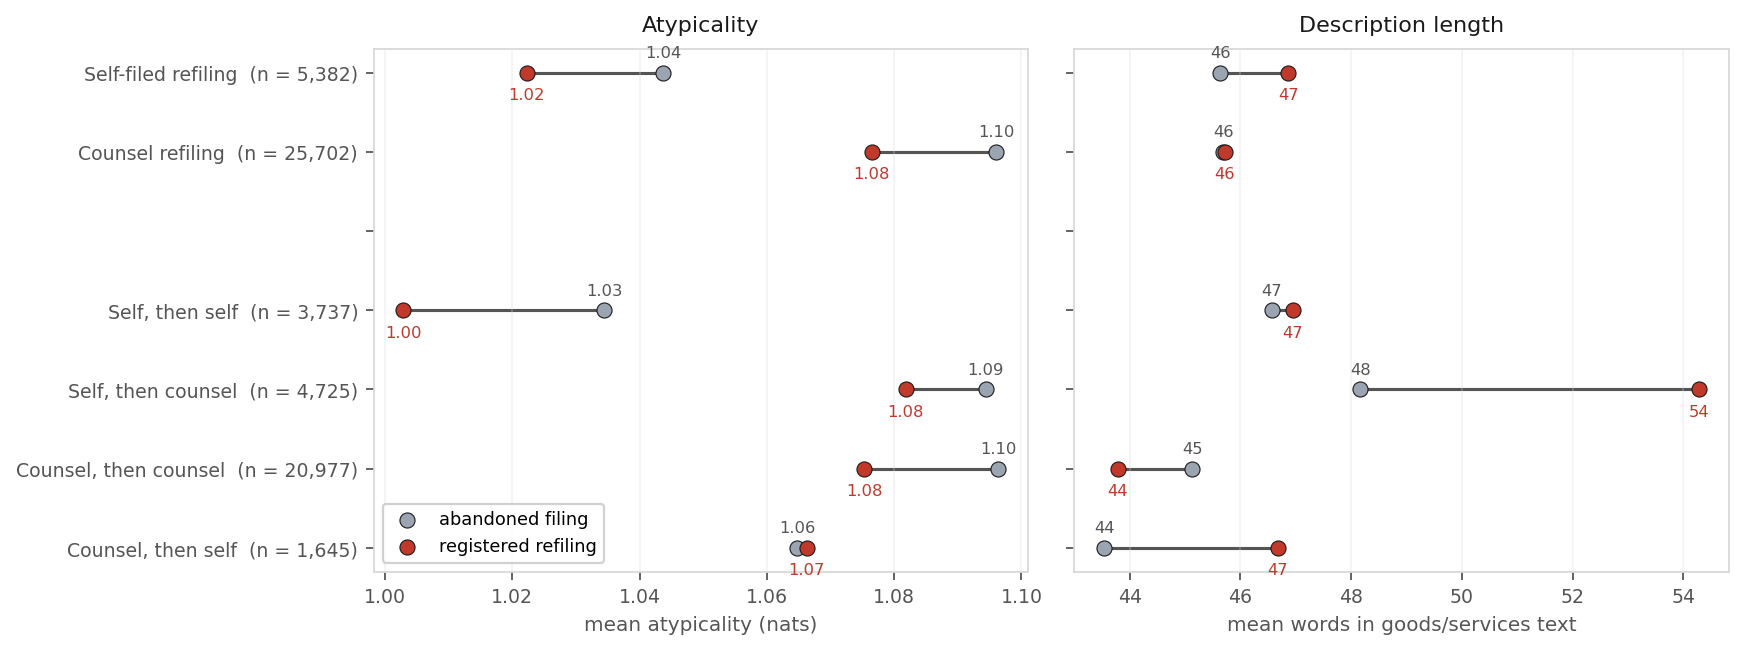
\includegraphics[width=\textwidth]{results/refile_prepost.png}
\caption{Rewritten refilings: mean atypicality and mean description length
of the abandoned filing (grey) and of the registered refiling (red), by
representation on the refiling and by the change in representation between
the two attempts. Mean atypicality falls by $0.01$ to $0.03$ nats in every
group except counsel-then-self, where it is unchanged; the means are small
because the convergence runs from both tails, which the profile by fifth
below shows. Length rises by six words where counsel is hired for the
second attempt and falls by one where counsel rewrites counsel.}
\label{fig:refile}
\end{figure}

The means understate the convergence, because it runs in both directions.
By fifth of the original's atypicality, the change is $+0.16$, $+0.14$,
$+0.06$, $-0.06$ and $-0.39$ nats from the most conventional fifth to the
most atypical, and within a point of that profile in each of the four
representation groups. Identical-text refilings change by $+0.002$ to
$+0.008$ across the same fifths. On lead, the changed-text profile runs
$+0.046$ to $-0.072$ and the identical-text profile $+0.014$ to $-0.054$;
the difference is the rewriting, the rest is the reference windows moving
with the later filing date.

\section{The outcome analysis without registration conditioning}\label{app:uncond}

Figure~\ref{fig:uncond} repeats the lifecycle outcome analysis without the
registration conditioning, on filings 2013--2015 pooled across all classes
(a window whose registrations land by $\sim$2017 and face at least one
Section~8 gate by the 2025 snapshot; the earliest registrations in the
window also face their year-ten renewal, so panel B mixes one and two
gates). Panel A is the unconditional composite, the probability that a
filing both registers and passes the gate, measured over all filings
including the never-registered. It is nearly flat in \dkl{} --- $22.4$\% at the bottom quintile against
$22.1$\% at the top, a middle-versus-tails depth of $+0.001$pp (SE $0.10$) ---
because two opposed gradients cancel: registration rises in lead
($61.3$\% to $63.2$\%) while gate survival falls ($44.2$\% to $40.8$\%).
Conditioning on grant is what separates them. Panel B shows the conditional
gate outcome on the same filings, and it is U-shaped rather than inverse-U
(depth $-2.11$pp), with a clearly penalised leading tail consistent with the
cleaner single-gate cohort of Figure~\ref{fig:s8pooled}.

\begin{figure}[h]\centering
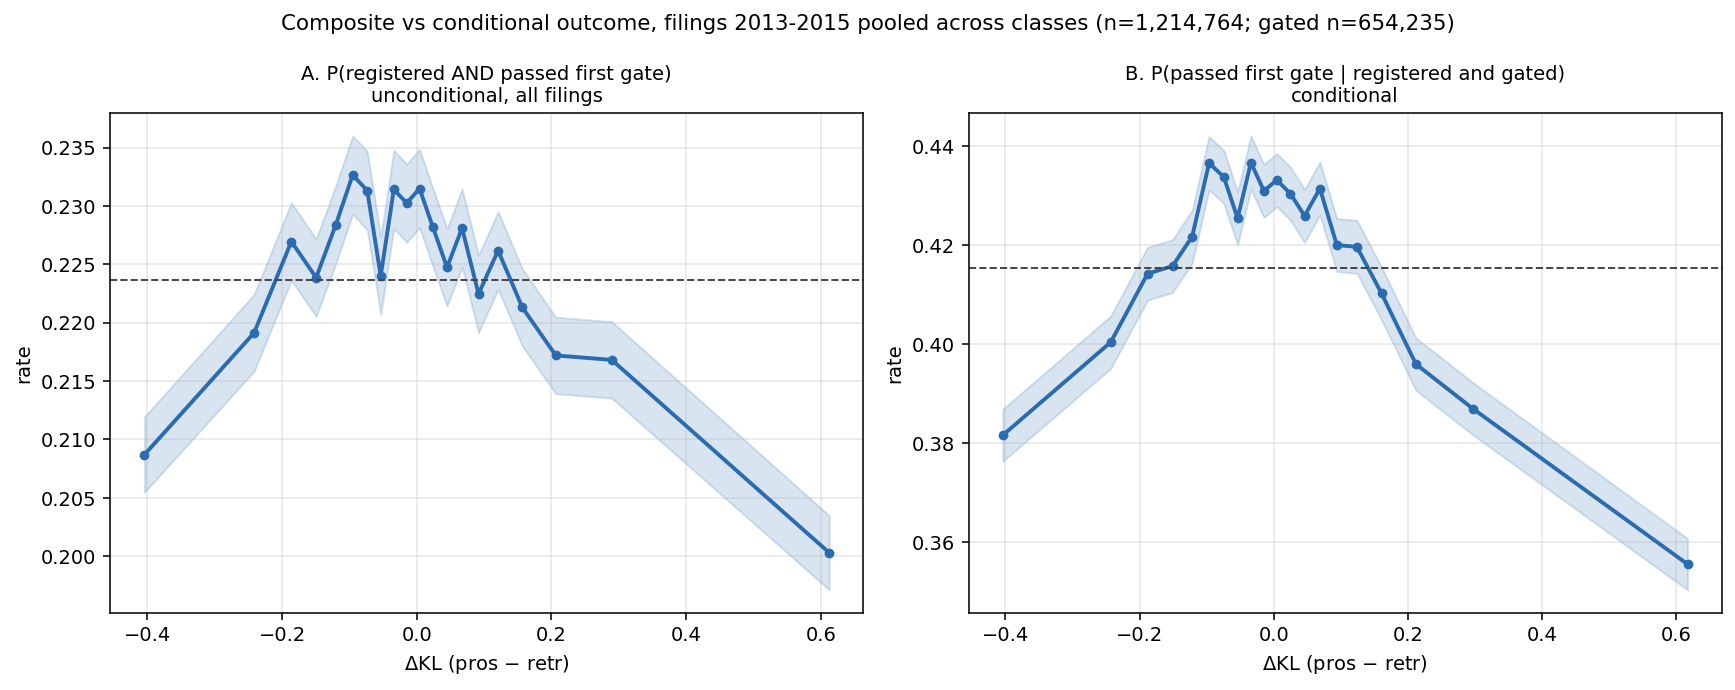
\includegraphics[width=\textwidth]{results/appendix_unconditional.png}
\caption{Filings 2013--2015 pooled across classes, topic-scored on
per-filing reference windows ($n = 1{,}419{,}678$; gated subset
$n = 763{,}902$). \emph{A:} the unconditional composite P(registered and
passed first gate) over all filings. \emph{B:} P(passed $\mid$ registered
and gated) on the same filings. The unconditional view is nearly flat in
lead (22.4\% to 22.1\% across quintiles); conditioning on grant is what
exposes the gradient.}
\label{fig:uncond}
\end{figure}

\section{Term scoring measures length; theme scoring does not}\label{app:representation}

Figure~\ref{fig:representation} puts the two representations side by side
over the same axes, with each hexagon coloured by the mean length of the
filings in it. Under term scoring the colour runs from dark near the
origin --- a median of about 200 terms --- to near-white at the far end,
where the median is eight. That gradient is the measurement problem: a
filing scores as atypical largely because it is short. Under topic scoring
the same surface is a narrow band of roughly uniform tone.

Two filings are marked in both columns. Under the production scoring they
behave differently from one another, which is the point. \textsc{Amazon.com}
(1997) is a leader on both representations --- the 98th percentile of its
class on terms and the 94th on themes --- while sitting at the 40th and 47th
percentiles of atypicality, so both agree that it was early and neither
mistakes it for strange. Apple's \textsc{iPod} (2001) divides them: the 31st
percentile of lead on terms against the 62nd on themes. The surfaces plotted
here are on the class-year build the figure was generated from, where the
length gradient is starkest; the percentiles just quoted are on the per-filing
build used for every estimate.

\begin{figure}[h]\centering
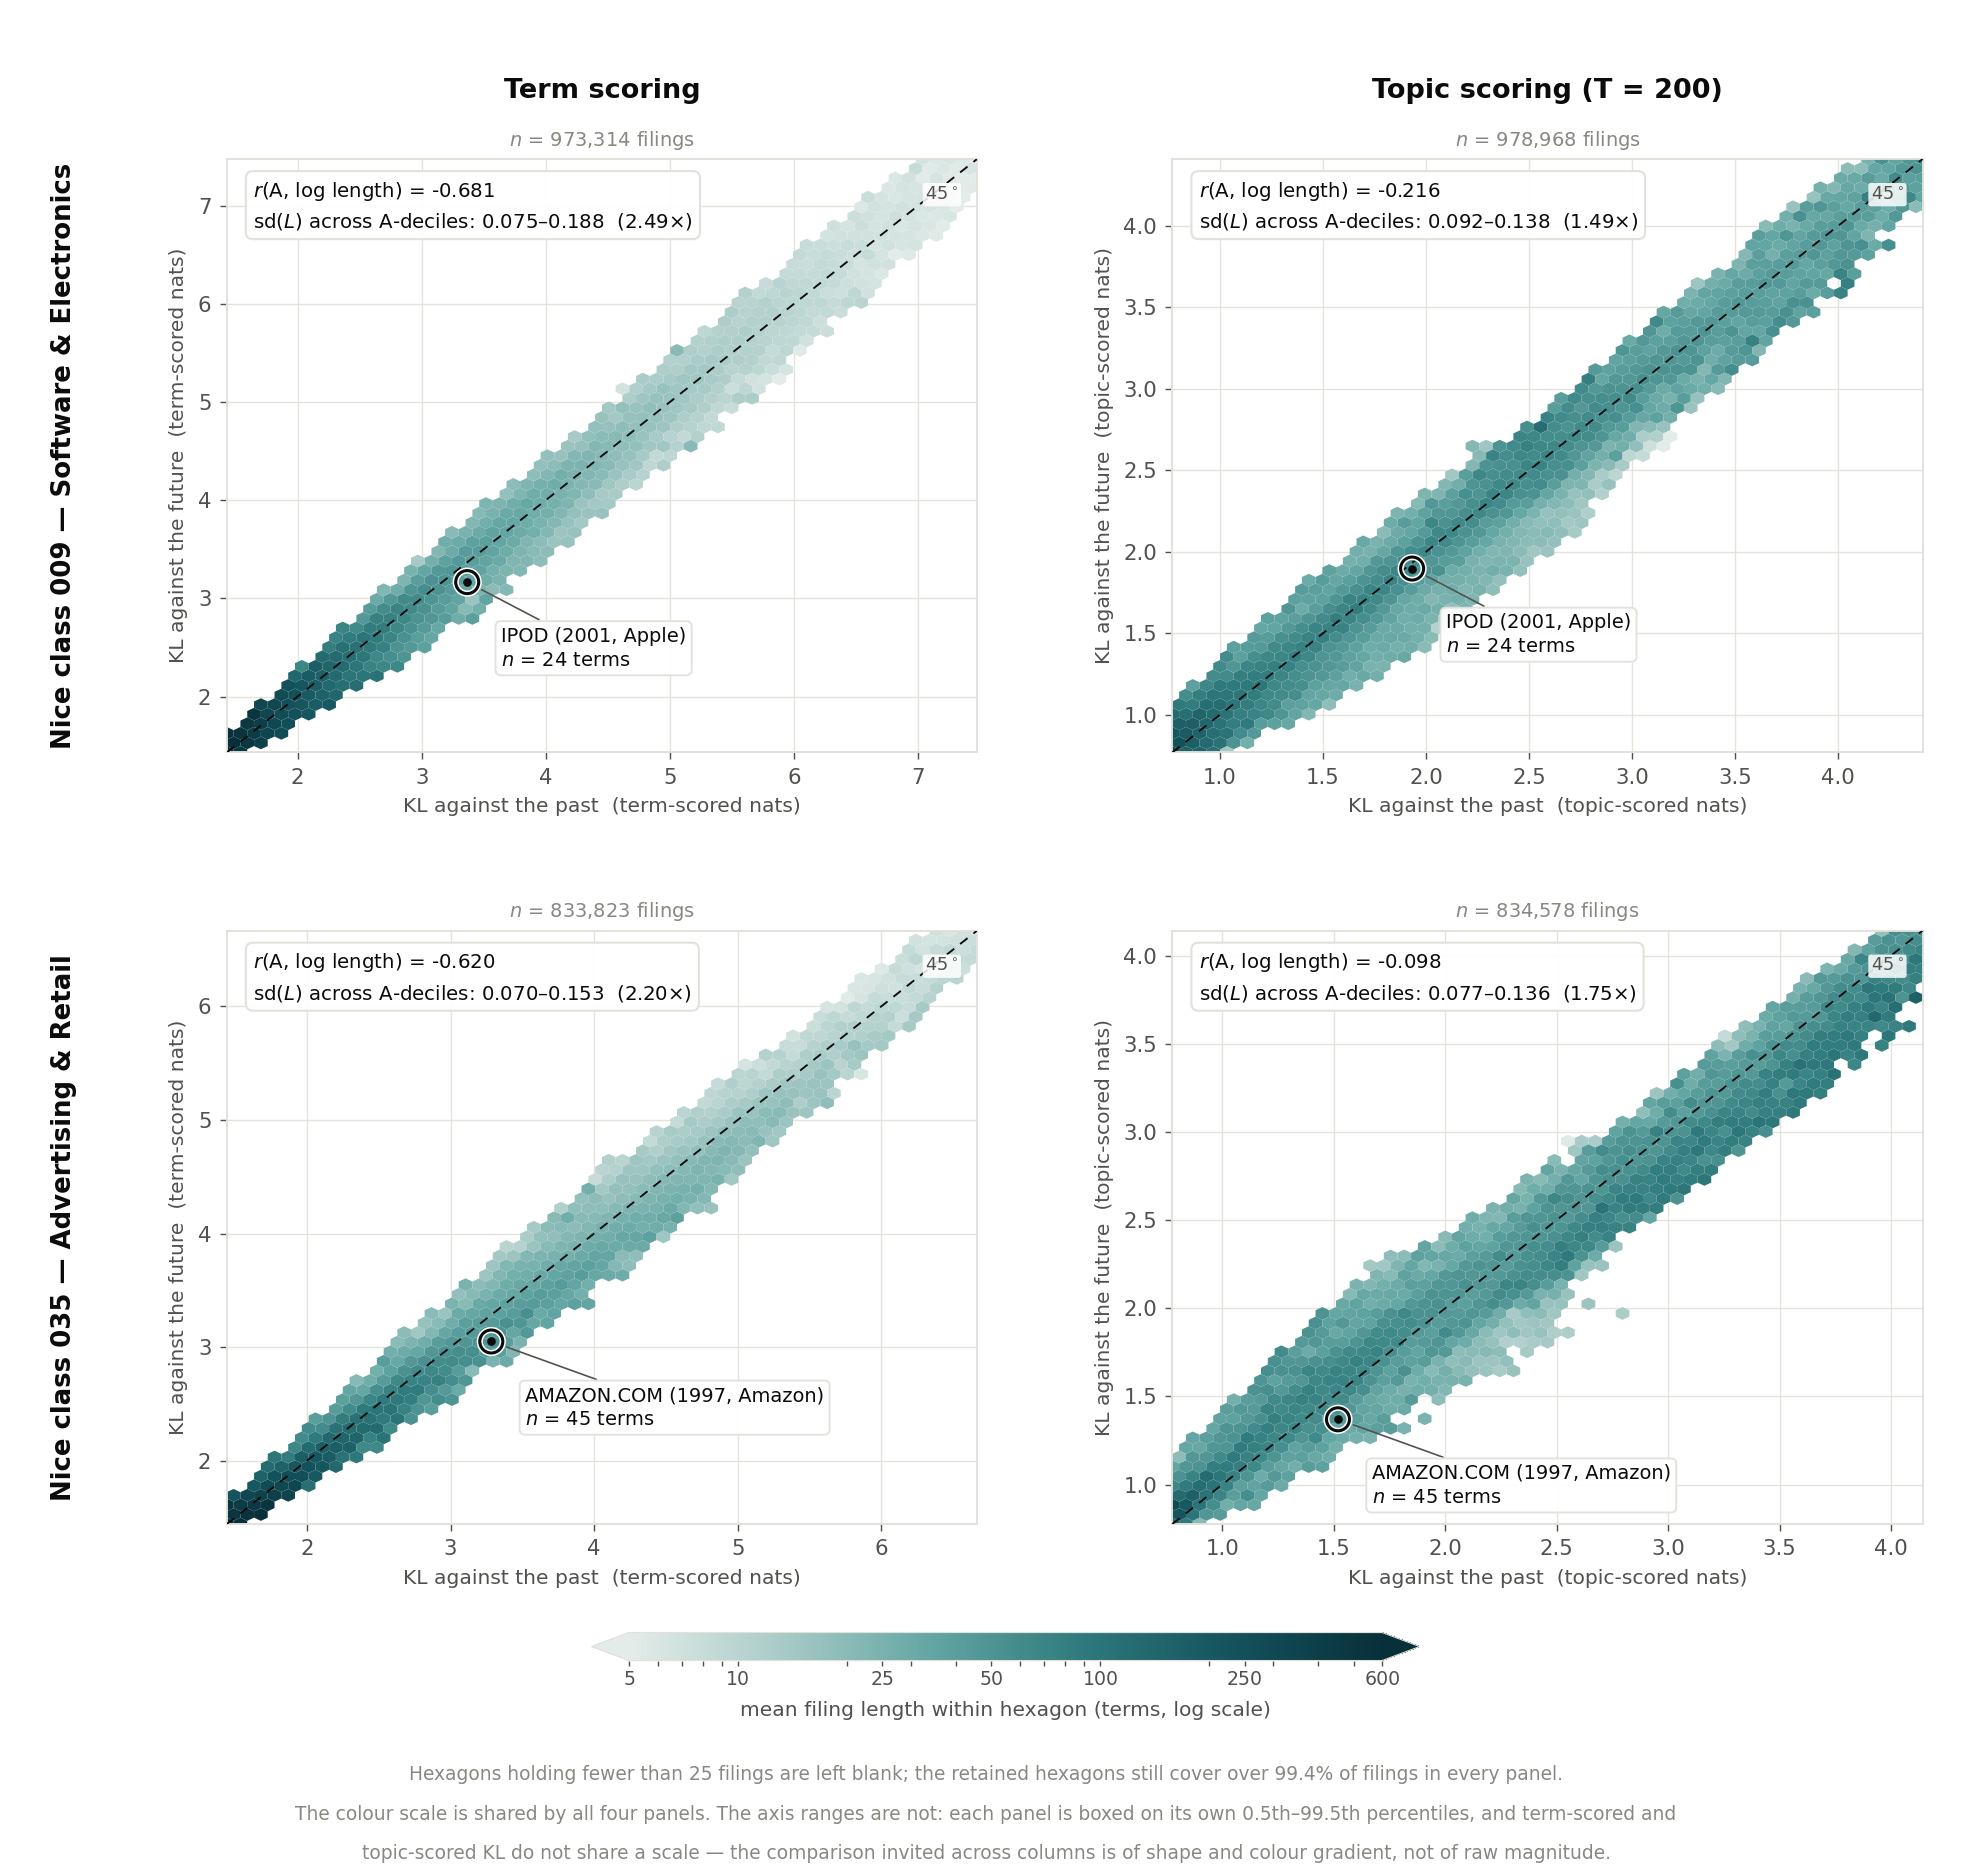
\includegraphics[width=\textwidth]{results/representation_appendix.png}
\caption{Mean filing length across the two axes, by representation and
class, for filings 1995--2019 scored on per-filing reference windows. The
horizontal axis is surprise against the preceding five years, the vertical
axis surprise against the following five; a filing on the dashed diagonal
is equally far from both, and distance below it is lead. Hexagons holding fewer than 25 filings are blank; the retained
hexagons cover over 99.4\% of filings in every panel. The colour scale is
shared across panels; the axis ranges are not, since term-scored and
topic-scored KL do not share a scale, so the comparison invited across
columns is of shape and colour gradient rather than of magnitude. Both
columns are drawn on the filings the per-filing windows score, which
differ between representations by under one percent.}
\label{fig:representation}
\end{figure}

Topic scoring is independent of document length, which term scoring is not; term scoring
resolves novel word \emph{combinations}, which topic scoring does not. Hence
topic scoring for every estimate, since the length confound contaminates
firm-level comparisons, and term scoring for every worked example, since the
topic basis has no coordinate for the language the examples turn on.

\section{How three filings encode}\label{app:exhibit}

Table~\ref{tab:exhibit} traces three filings through term scoring and topic
scoring at $T \in \{50, 200, 500\}$ --- three kinds of novelty, and how each
representation handles them.

\textsc{Amazon.com} (1997, advertising/retail) is \emph{combinatorial}
novelty: every word is ordinary, but the bigrams assemble an invention
(``computerized line,'' ``line search,'' ``search ordering''; class
document frequencies 379, 134, 355). The filing's text reads ``on line''
as two words, the standard spelling in 1997, before \emph{online}
lexicalized into a single token; the analyzer drops the stopword ``on''
and the surviving bigram ``line search'' is the act of forming the
compound caught in progress. The novelty was necessarily combinatorial
because the word for it did not yet exist. Term scoring sees these
bigrams; under topic scoring at every resolution all of them are out of
vocabulary and the filing reads as a media retailer that uses computers.

\textsc{Kombucha} (1997, beer/soft drinks) is \emph{lexical} novelty: the
new thing arrives as new words (\emph{kombucha} df 567, \emph{saccharose}
out of vocabulary even at the class level). The word \emph{kombucha} is in
the topic vocabulary but, with no kombucha-like topic, its mass dissolves
into a generic beverages topic ($\geq 0.60$ weight at every $T$).

\textsc{Ethereum} (2018, software) is \emph{wave} novelty: emergent
vocabulary already diffusing (\emph{blockchains}, \emph{distributed
computing}). It loads on generic software and services topics at every
resolution, including $T = 200$, which does contain a
cryptocurrency/blockchain topic --- the eleven occurrences of
\emph{software} outvote the blockchain terms.

\begin{table}[h]\centering\small
\caption{Top topic loading for three filings, by representation. Term
scoring resolves the novel content of all three; topic scoring resolves
none of it at any tested resolution.}
\label{tab:exhibit}
\begin{tabular}{lp{3.1cm}p{3.1cm}p{3.1cm}}
\toprule
& \textsc{Amazon.com} & \textsc{Kombucha} & \textsc{Ethereum} \\
& (1997) & (1997) & (2018) \\
\midrule
novel content (term) & line search, search ordering & kombucha, saccharose & blockchains, distributed computing \\
$T=50$ & video, computer, music (0.40) & beverages, fruit, drinks (0.64) & software, online, downloadable (0.33) \\
$T=200$ & entertainment, video, games (0.29) & beverages, drinks, coffee (0.60) & field, services, development (0.37) \\
$T=500$ & computer, software, data (0.22) & beverages, drinks, fruit (0.61) & software, online, computer (0.49) \\
\bottomrule
\end{tabular}
\end{table}

The pattern across the row is the measurement point in miniature: topic
scoring cannot represent combinatorial novelty (Amazon), dilutes lexical
novelty (Kombucha), and majority-votes away wave novelty (Ethereum) even
when a fitting topic exists. That the mark-level outcome results are
nearly identical under both scorings despite this blindness is what
licenses topic scoring as a robustness instrument; that the firm-level
results diverge is what exposes them as artifacts of the lexical
specificity term scoring additionally captures
(Appendix~\ref{app:hazard}).

